\documentclass{standalone}
\usepackage{tikz}
\usepackage{amsmath}

\usetikzlibrary{arrows.meta,decorations.pathreplacing}

\tikzset{
    line/.style={
        thick
    },
    arrow/.style={
        line,
        ->,
        > = {
            Triangle[length=2.0mm, width=2.0mm]
        }
    }
}

% Switch to Sans Serif font.
\renewcommand{\familydefault}{\sfdefault}

\renewcommand{\wedge}{$\vphantom{\big|}$}


\newcommand{\lineat}[4]{
    \draw [#4] ({#1}, 0) -- ({#1}, -0.5);
    \draw [black!10, fill=black!10]
        ({#1 - #2}, 1) --
        ({#1}, 0) --
        ({#1 + #3}, 1);
}

\begin{document}
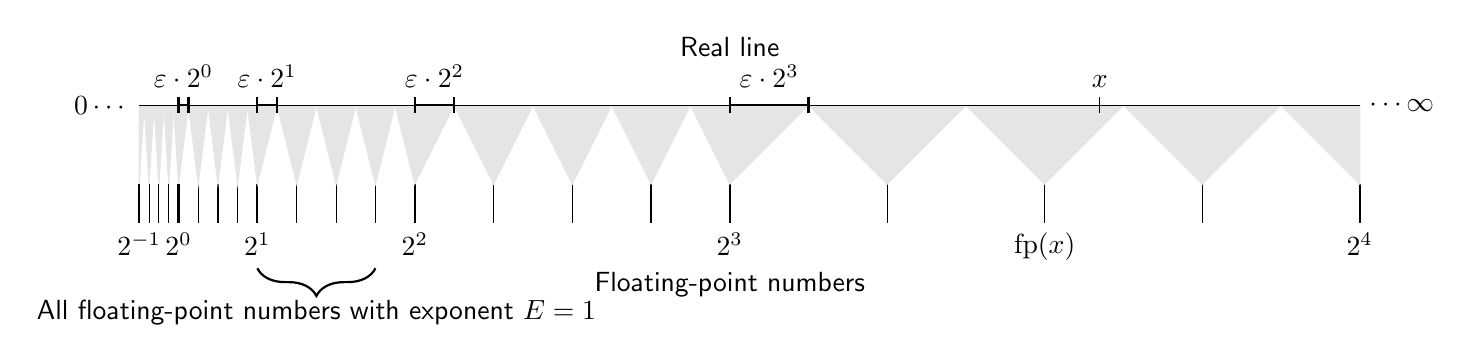
\begin{tikzpicture}[xscale=1]
    \lineat
        {2^-1}
        {0}
        {2^(-1 - 3)}{thick}
    \node [anchor=north] () at (2^-1, -0.5) {$2^{-1}$};
    \foreach \i in {1, ..., 3} {
        \lineat
            {2^-1 + \i * 2^(-1 - 2)}
            {2^(-1 - 3)}
            {2^(-1 - 3)}{}
    }
    \foreach \start in {0, 1, 2, 3} {
        \lineat
            {2^\start}
            {2^(\start - 4)}
            {2^(\start - 3)}{thick}
        \node [anchor=north] () at (2^\start, -0.5) {$2^{\start}$};
        \foreach \i in {1, ..., 3} {
            \lineat
                {2^\start + \i * 2^(\start - 2)}
                {2^(\start - 3)}
                {2^(\start - 3)}{}
        }
    }
    \lineat{2^4}{2^(4 - 4)}{0}{thick}
    \node [anchor=north] () at (2^4, -0.5) {$2^4$};
    \draw (2^-1, 1) -- (2^4, 1);
    \node [anchor=south] () at (2^4 / 2, 1.5) {Real line};
    \node [anchor=north] () at (2^4 / 2, -1) {Floating-point numbers};
    \node [anchor=east] () at (2^-1, 1) {$0 \cdots$};
    \node [anchor=west] () at (2^4, 1) {$\cdots \infty$};

    \foreach \start in {0, 1, 2, 3} {
        \draw [thick] (2^\start, 1 - 0.1) -- (2^\start, 1 + 0.1);
        \draw [thick] ({2^\start + 0.5 * 2^(\start - 2)}, 1 - 0.1) -- ({2^\start + 0.5 * 2^(\start - 2)}, 1 + 0.1);
        \draw [thick] (2^\start, 1) -- ({2^\start + 0.5 * 2^(\start - 2)}, 1);
        \node [anchor=south] () at ({2^\start + 0.25 * 2^(\start - 2)}, 1 + 0.1) {$\varepsilon \cdot 2^{\start}$};
    }

    \draw [
        thick,
        decorate,
        decoration={brace,amplitude=10pt,mirror,raise=2pt},
        yshift=0pt
    ]
        (2^1, -1) -- ({2^1 + 3 * 2^(1 - 2)}, -1)
        node [black, midway, anchor=north, yshift=-10pt] {All floating-point numbers with exponent $E=1$};

    \draw ({2^3 + 2.35 * 2^(3 - 2)}, 0.9) -- ({2^3 + 2.35 * 2^(3 - 2)}, 1.1) node [anchor=south, pos=1] {$x$};
    \node [anchor=north] () at ({2^3 + 2 * 2^(3 - 2)}, -0.5) {$\operatorname{fp}(x)$};
\end{tikzpicture}
\end{document}